% Options for packages loaded elsewhere
\PassOptionsToPackage{unicode}{hyperref}
\PassOptionsToPackage{hyphens}{url}
\PassOptionsToPackage{dvipsnames,svgnames*,x11names*}{xcolor}
%
\documentclass[
  english,
  man,floatsintext]{apa6}
\usepackage{lmodern}
\usepackage{amssymb,amsmath}
\usepackage{ifxetex,ifluatex}
\ifnum 0\ifxetex 1\fi\ifluatex 1\fi=0 % if pdftex
  \usepackage[T1]{fontenc}
  \usepackage[utf8]{inputenc}
  \usepackage{textcomp} % provide euro and other symbols
\else % if luatex or xetex
  \usepackage{unicode-math}
  \defaultfontfeatures{Scale=MatchLowercase}
  \defaultfontfeatures[\rmfamily]{Ligatures=TeX,Scale=1}
\fi
% Use upquote if available, for straight quotes in verbatim environments
\IfFileExists{upquote.sty}{\usepackage{upquote}}{}
\IfFileExists{microtype.sty}{% use microtype if available
  \usepackage[]{microtype}
  \UseMicrotypeSet[protrusion]{basicmath} % disable protrusion for tt fonts
}{}
\makeatletter
\@ifundefined{KOMAClassName}{% if non-KOMA class
  \IfFileExists{parskip.sty}{%
    \usepackage{parskip}
  }{% else
    \setlength{\parindent}{0pt}
    \setlength{\parskip}{6pt plus 2pt minus 1pt}}
}{% if KOMA class
  \KOMAoptions{parskip=half}}
\makeatother
\usepackage{xcolor}
\IfFileExists{xurl.sty}{\usepackage{xurl}}{} % add URL line breaks if available
\IfFileExists{bookmark.sty}{\usepackage{bookmark}}{\usepackage{hyperref}}
\hypersetup{
  pdftitle={Epidemiologische situatie COVID-19 in Nederland - 09 augustus 2021},
  pdfauthor={Marino van Zelst1},
  pdflang={en-EN},
  colorlinks=true,
  linkcolor=Maroon,
  filecolor=Maroon,
  citecolor=Blue,
  urlcolor=blue,
  pdfcreator={LaTeX via pandoc}}
\urlstyle{same} % disable monospaced font for URLs
\usepackage{graphicx,grffile}
\makeatletter
\def\maxwidth{\ifdim\Gin@nat@width>\linewidth\linewidth\else\Gin@nat@width\fi}
\def\maxheight{\ifdim\Gin@nat@height>\textheight\textheight\else\Gin@nat@height\fi}
\makeatother
% Scale images if necessary, so that they will not overflow the page
% margins by default, and it is still possible to overwrite the defaults
% using explicit options in \includegraphics[width, height, ...]{}
\setkeys{Gin}{width=\maxwidth,height=\maxheight,keepaspectratio}
% Set default figure placement to htbp
\makeatletter
\def\fps@figure{htbp}
\makeatother
\setlength{\emergencystretch}{3em} % prevent overfull lines
\providecommand{\tightlist}{%
  \setlength{\itemsep}{0pt}\setlength{\parskip}{0pt}}
\setcounter{secnumdepth}{-\maxdimen} % remove section numbering
% Make \paragraph and \subparagraph free-standing
\ifx\paragraph\undefined\else
  \let\oldparagraph\paragraph
  \renewcommand{\paragraph}[1]{\oldparagraph{#1}\mbox{}}
\fi
\ifx\subparagraph\undefined\else
  \let\oldsubparagraph\subparagraph
  \renewcommand{\subparagraph}[1]{\oldsubparagraph{#1}\mbox{}}
\fi
% Manuscript styling
\usepackage{upgreek}
\captionsetup{font=singlespacing,justification=justified}

% Table formatting
\usepackage{longtable}
\usepackage{lscape}
% \usepackage[counterclockwise]{rotating}   % Landscape page setup for large tables
\usepackage{multirow}		% Table styling
\usepackage{tabularx}		% Control Column width
\usepackage[flushleft]{threeparttable}	% Allows for three part tables with a specified notes section
\usepackage{threeparttablex}            % Lets threeparttable work with longtable

% Create new environments so endfloat can handle them
% \newenvironment{ltable}
%   {\begin{landscape}\begin{center}\begin{threeparttable}}
%   {\end{threeparttable}\end{center}\end{landscape}}
\newenvironment{lltable}{\begin{landscape}\begin{center}\begin{ThreePartTable}}{\end{ThreePartTable}\end{center}\end{landscape}}

% Enables adjusting longtable caption width to table width
% Solution found at http://golatex.de/longtable-mit-caption-so-breit-wie-die-tabelle-t15767.html
\makeatletter
\newcommand\LastLTentrywidth{1em}
\newlength\longtablewidth
\setlength{\longtablewidth}{1in}
\newcommand{\getlongtablewidth}{\begingroup \ifcsname LT@\roman{LT@tables}\endcsname \global\longtablewidth=0pt \renewcommand{\LT@entry}[2]{\global\advance\longtablewidth by ##2\relax\gdef\LastLTentrywidth{##2}}\@nameuse{LT@\roman{LT@tables}} \fi \endgroup}

% \setlength{\parindent}{0.5in}
% \setlength{\parskip}{0pt plus 0pt minus 0pt}

% \usepackage{etoolbox}
\makeatletter
\patchcmd{\HyOrg@maketitle}
  {\section{\normalfont\normalsize\abstractname}}
  {\section*{\normalfont\normalsize\abstractname}}
  {}{\typeout{Failed to patch abstract.}}
\patchcmd{\HyOrg@maketitle}
  {\section{\protect\normalfont{\@title}}}
  {\section*{\protect\normalfont{\@title}}}
  {}{\typeout{Failed to patch title.}}
\makeatother
\shorttitle{Dagelijkse rapportage}
\DeclareDelayedFloatFlavor{ThreePartTable}{table}
\DeclareDelayedFloatFlavor{lltable}{table}
\DeclareDelayedFloatFlavor*{longtable}{table}
\makeatletter
\renewcommand{\efloat@iwrite}[1]{\immediate\expandafter\protected@write\csname efloat@post#1\endcsname{}}
\makeatother
\usepackage{csquotes}
\ifxetex
  % Load polyglossia as late as possible: uses bidi with RTL langages (e.g. Hebrew, Arabic)
  \usepackage{polyglossia}
  \setmainlanguage[]{english}
\else
  \usepackage[shorthands=off,main=english]{babel}
\fi

\title{Epidemiologische situatie COVID-19 in Nederland - 09 augustus 2021}
\author{Marino van Zelst\textsuperscript{1}}
\date{}


\affiliation{\vspace{0.5cm}\textsuperscript{1} Vragen over deze rapportage kunnen verstuurd worden aan Marino van Zelst, twitter.com/mzelst. E-mail: \href{mailto:j.m.vanzelst@uvt.nl}{\nolinkurl{j.m.vanzelst@uvt.nl}}}

\begin{document}
\maketitle

{
\hypersetup{linkcolor=}
\setcounter{tocdepth}{3}
\tableofcontents
}
\newpage

\hypertarget{samenvatting}{%
\section{Samenvatting}\label{samenvatting}}

\textbf{Samenvatting (op basis van GGD cijfers)}\\
Tot en met 2021-08-09 zijn er in Nederland in totaal 1887831 COVID-19 patiënten gemeld aan het RIVM. Tot nu toe zijn 31583 van de gemelde patiënten opgenomen in het ziekenhuis en 17871 mensen overleden.

\textbf{Gegevens t. o. v. gisteren}\\
Positief getest: 2077
Totaal: 1887831 (+ 2026 ivm -51 corr.)

Opgenomen: 25
Totaal: 31583 (+
25 ivm 0 corr.)

Overleden: 2
Totaal: 17871 (+
2 ivm 0 corr.)

\textbf{Update met betrekking tot ziekenhuis-gegevens (data NICE)}

Patiënten verpleegafdeling\\
Bevestigd: 2 Verdacht: 4

Patiënten IC\\
Bevestigd: 6 Verdacht: 0

\textbf{Data}\\
Een databestand met de cumulatieve aantallen per gemeente per dag van gemelde COVID-19 patiënten, in het ziekenhuis opgenomen COVID-19 patiënten en overleden COVID-19 patiënten is \href{https://data.rivm.nl/geonetwork/srv/dut/catalog.search\#/metadata/1c0fcd57-1102-4620-9cfa-441e93ea5604}{hier} te vinden. Een databestand met karakteristieken van elke positief geteste COVID-19 patiënt in Nederland is \href{https://data.rivm.nl/geonetwork/srv/dut/catalog.search\#/metadata/2c4357c8-76e4-4662-9574-1deb8a73f724?tab=relations}{hier} te vinden. Alle gegevens die voor dit rapport gebruikt worden zijn te vinden in de \href{https://github.com/mzelst/covid-19}{Github repository}.

\newpage

\hypertarget{covid-19-meldingen-in-de-afgelopen-vier-weken}{%
\section{COVID-19 meldingen in de afgelopen vier weken}\label{covid-19-meldingen-in-de-afgelopen-vier-weken}}

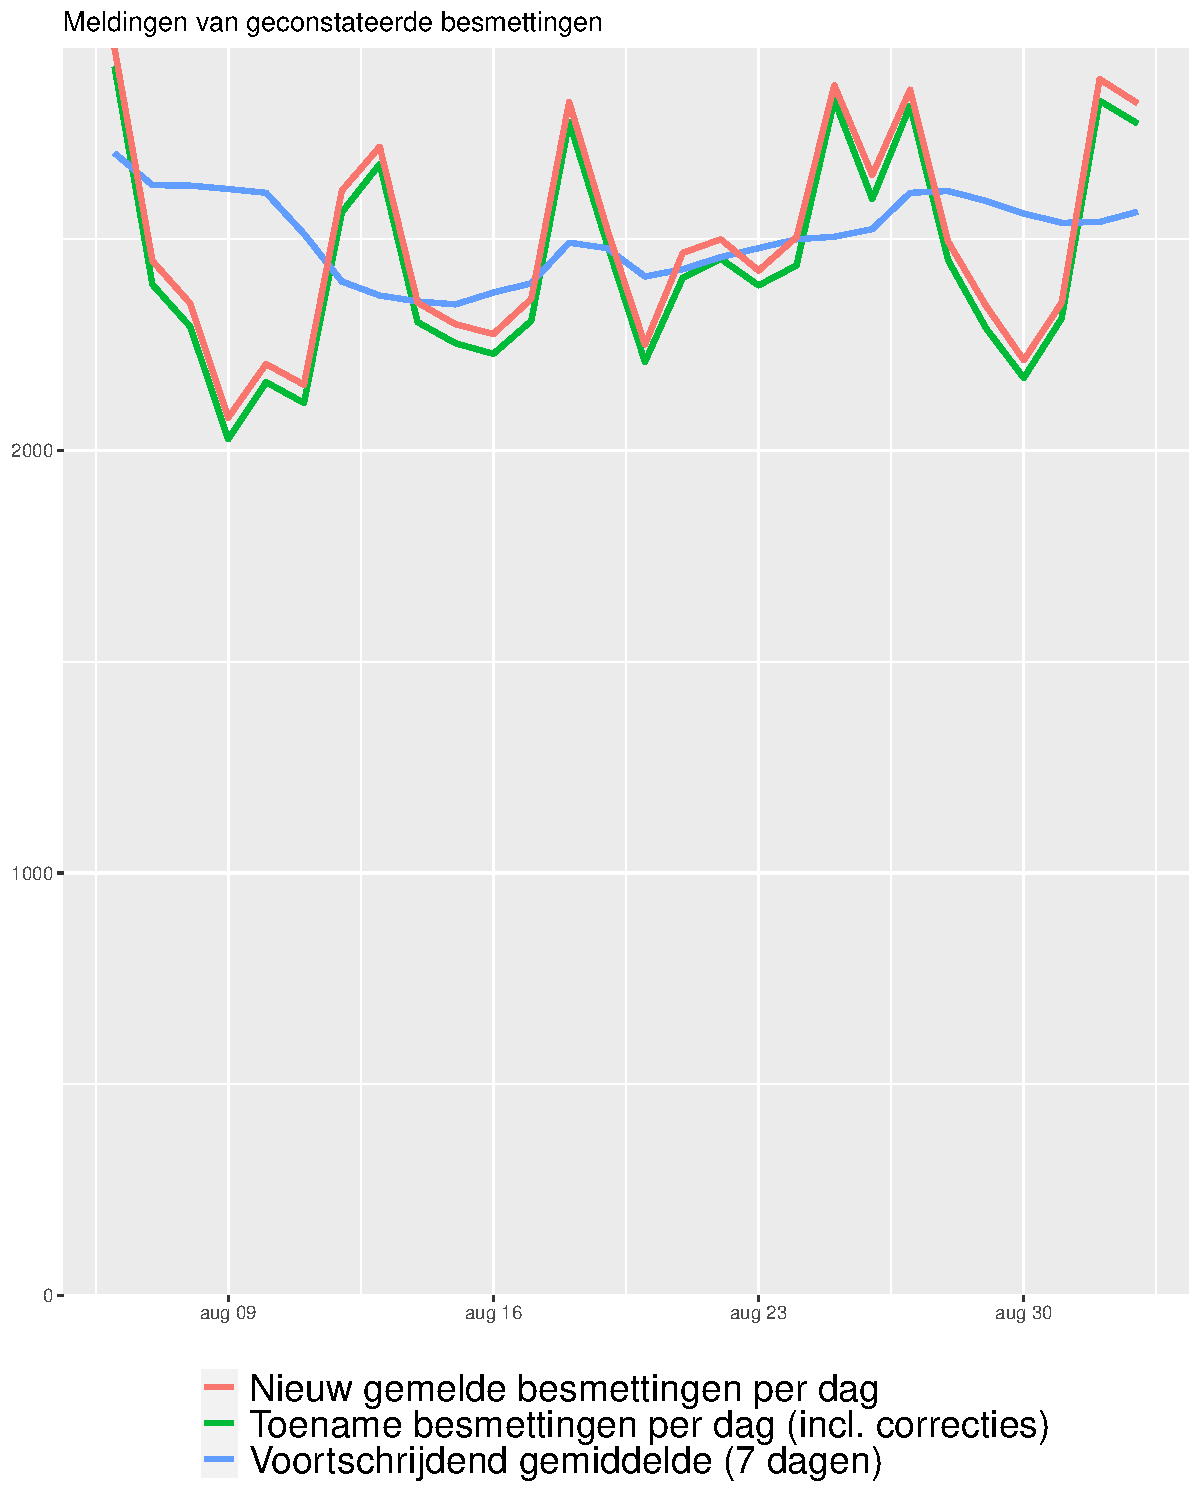
\includegraphics{daily_report_files/figure-latex/Gemelde besmettingen-1.pdf}

\newpage

\hypertarget{kaart-met-covid-19-meldingen-per-gemeente-sinds-gisteren}{%
\section{Kaart met COVID-19 meldingen per gemeente sinds gisteren}\label{kaart-met-covid-19-meldingen-per-gemeente-sinds-gisteren}}

\begin{figure}
\centering
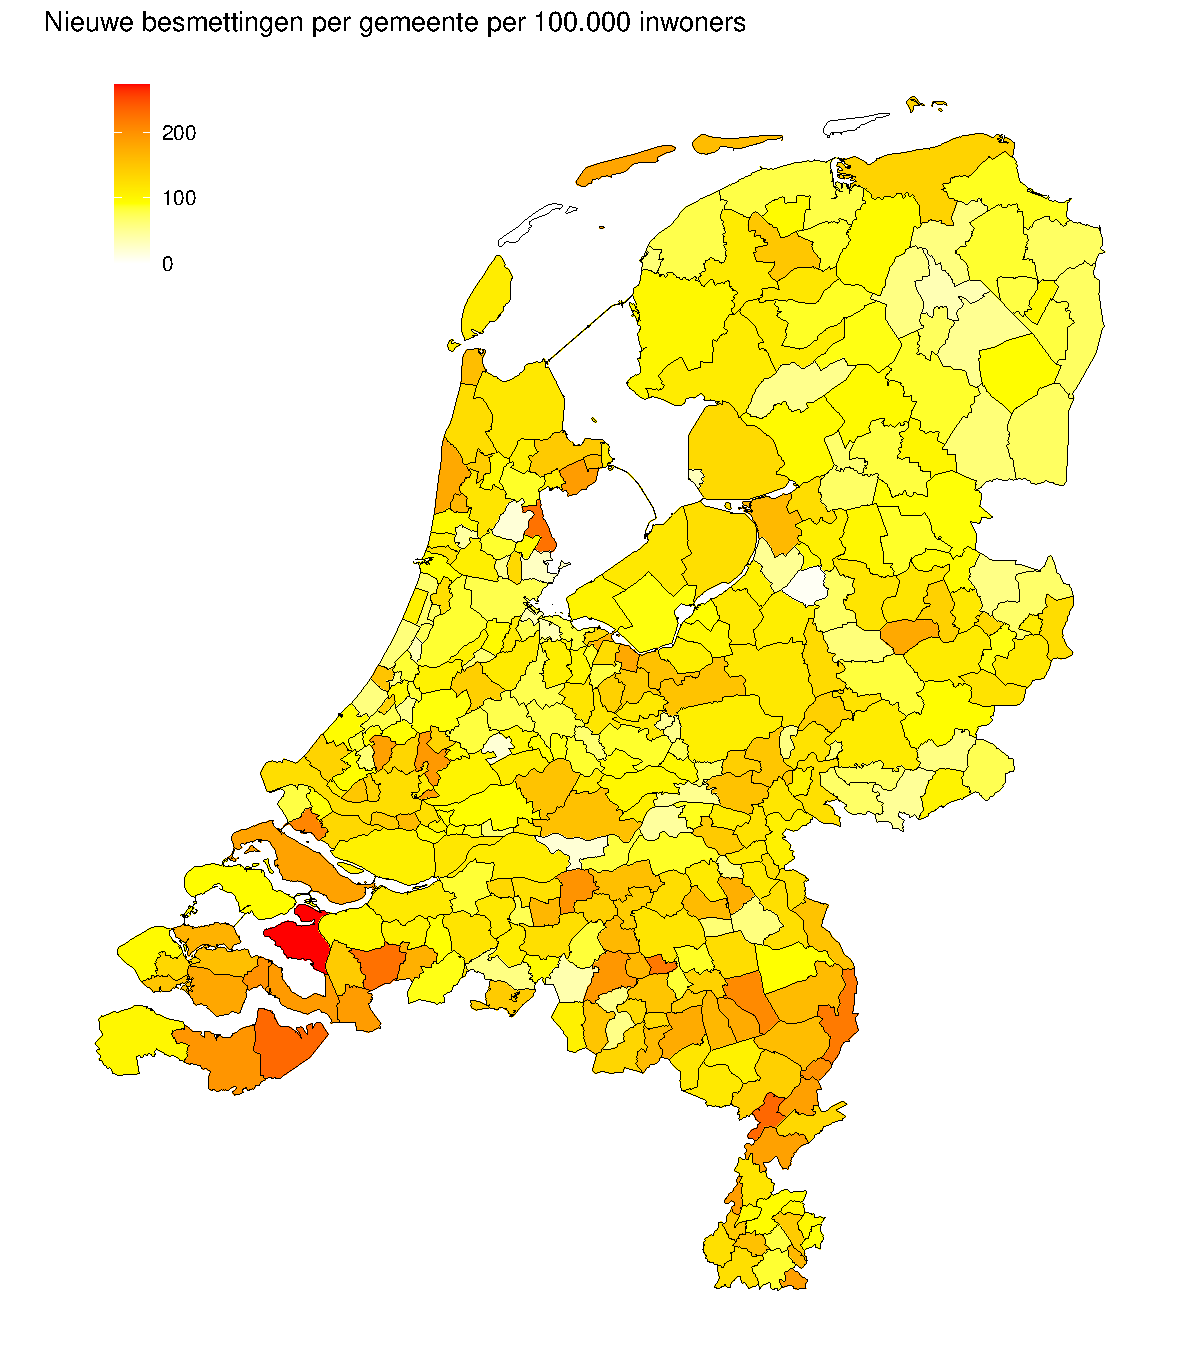
\includegraphics{daily_report_files/figure-latex/Gemeentes - sinds gisteren-1.pdf}
\caption{(\#Gemeentes - sinds gisteren) Aantal, sinds gisteren, bij de GGD'en gemelde COVID-19 patiënten per 100.000 inwoners per gemeente}
\end{figure}

\newpage

\hypertarget{kaart-met-covid-19-meldingen-per-gemeente-in-de-afgelopen-week}{%
\section{Kaart met COVID-19 meldingen per gemeente in de afgelopen week}\label{kaart-met-covid-19-meldingen-per-gemeente-in-de-afgelopen-week}}

\begin{figure}
\centering
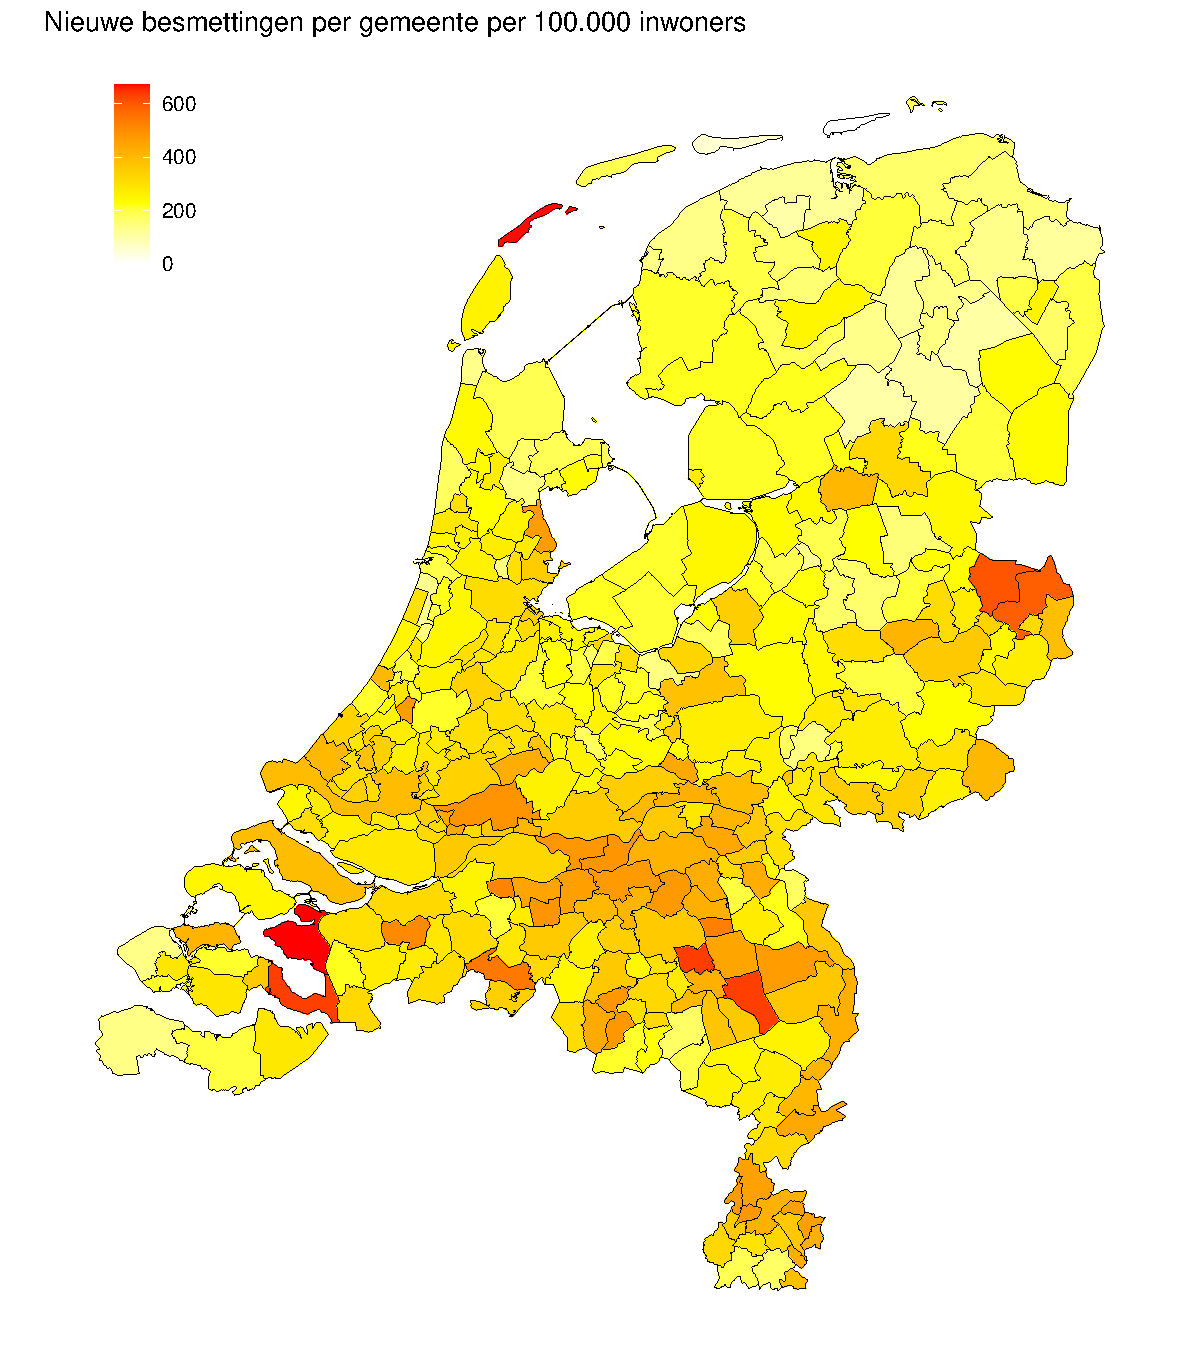
\includegraphics{daily_report_files/figure-latex/Gemeentes - Sinds vorige week-1.pdf}
\caption{(\#Gemeentes - Sinds vorige week) Aantal in de afgelopen week bij de GGD'en gemelde COVID-19 patiënten per 100.000 inwoners per gemeente.}
\end{figure}

\newpage

\hypertarget{aantal-covid-19-meldingen-per-provincie-in-de-afgelopen-twee-weken}{%
\section{Aantal COVID-19 meldingen per provincie in de afgelopen twee weken}\label{aantal-covid-19-meldingen-per-provincie-in-de-afgelopen-twee-weken}}

\begin{table}
\centering
\begin{threeparttable}
\begin{tabular}{lrrrrrr}
\toprule
\multicolumn{1}{c}{ } & \multicolumn{2}{c}{Besmettingen} & \multicolumn{2}{c}{Ziekenhuisopnames} & \multicolumn{2}{c}{Overleden} \\
\cmidrule(l{3pt}r{3pt}){2-3} \cmidrule(l{3pt}r{3pt}){4-5} \cmidrule(l{3pt}r{3pt}){6-7}
Provincie & Totaal & /100000 & Totaal & /100000 & Totaal & /100000\\
\midrule
Drenthe & 598 & 120.6 & 4 & 0.8 & 0 & 0.0\\
Flevoland & 1210 & 280.9 & 19 & 4.4 & 3 & 0.7\\
Fryslân & 1210 & 185.6 & 14 & 2.1 & 4 & 0.6\\
Gelderland & 4068 & 193.7 & 22 & 1.0 & 9 & 0.4\\
Groningen & 1066 & 181.6 & 8 & 1.4 & 2 & 0.3\\
Limburg & 2880 & 258.1 & 26 & 2.3 & 8 & 0.7\\
Noord-Brabant & 5888 & 228.4 & 36 & 1.4 & 3 & 0.1\\
Noord-Holland & 7817 & 270.6 & 99 & 3.4 & 19 & 0.7\\
Overijssel & 2585 & 221.4 & 17 & 1.5 & 2 & 0.2\\
Utrecht & 2615 & 191.9 & 46 & 3.4 & 6 & 0.4\\
Zeeland & 744 & 192.9 & 6 & 1.6 & 0 & 0.0\\
Zuid-Holland & 9778 & 262.1 & 99 & 2.7 & 14 & 0.4\\
\bottomrule
\end{tabular}
\begin{tablenotes}
\item \textit{Note: } 
\item Aantal bij de GGD’en gemelde COVID-19 patiënten, in het ziekenhuis opgenomen COVID-19 patiënten en overleden COVID-19 patiënten per provincie van 26 juli t/m 09 augustus 10:00 uur, totaal en per 100.000 inwoners
\end{tablenotes}
\end{threeparttable}
\end{table}

\newpage

\hypertarget{aantal-covid-19-meldingen-per-ggd-in-de-afgelopen-twee-weken}{%
\section{Aantal COVID-19 meldingen per GGD in de afgelopen twee weken}\label{aantal-covid-19-meldingen-per-ggd-in-de-afgelopen-twee-weken}}

\begin{table}
\centering\begingroup\fontsize{10}{12}\selectfont

\begin{threeparttable}
\begin{tabular}{lrrrrrr}
\toprule
\multicolumn{1}{c}{ } & \multicolumn{2}{c}{Besmettingen} & \multicolumn{2}{c}{Ziekenhuisopnames} & \multicolumn{2}{c}{Overleden} \\
\cmidrule(l{3pt}r{3pt}){2-3} \cmidrule(l{3pt}r{3pt}){4-5} \cmidrule(l{3pt}r{3pt}){6-7}
GGD & Totaal & /100000 & Totaal & /100000 & Totaal & /100000\\
\midrule
Dienst Gezondheid \& Jeugd ZHZ & 965 & 209.0 & 3 & 0.6 & 1 & 0.2\\
GGD Amsterdam & 3807 & 355.6 & 68 & 6.4 & 10 & 0.9\\
GGD Brabant-Zuidoost & 1817 & 231.3 & 11 & 1.4 & 1 & 0.1\\
GGD Drenthe & 606 & 122.2 & 4 & 0.8 & 0 & 0.0\\
GGD Flevoland & 1216 & 282.1 & 19 & 4.4 & 3 & 0.7\\
GGD Fryslân & 1219 & 186.9 & 14 & 2.1 & 4 & 0.6\\
GGD Gelderland-Zuid & 1044 & 184.7 & 8 & 1.4 & 2 & 0.4\\
GGD Gooi en Vechtstreek & 578 & 222.7 & -1 & -0.4 & 3 & 1.2\\
GGD Groningen & 984 & 167.7 & 7 & 1.2 & 2 & 0.3\\
GGD Haaglanden & 3101 & 275.7 & 43 & 3.8 & 6 & 0.5\\
GGD Hart voor Brabant & 2575 & 238.0 & 11 & 1.0 & 1 & 0.1\\
GGD Hollands-Midden & 1753 & 214.7 & 11 & 1.3 & 4 & 0.5\\
GGD Hollands-Noorden & 1410 & 211.2 & 7 & 1.0 & 4 & 0.6\\
GGD IJsselland & 1020 & 190.3 & 6 & 1.1 & 0 & 0.0\\
GGD Kennemerland & 1268 & 229.7 & 12 & 2.2 & 2 & 0.4\\
GGD Limburg-Noord & 1215 & 232.5 & 6 & 1.1 & 2 & 0.4\\
GGD Noord- en Oost-Gelderland & 1597 & 191.7 & 5 & 0.6 & 4 & 0.5\\
GGD Regio Utrecht & 2619 & 414.6 & 46 & 7.3 & 6 & 0.9\\
GGD Rotterdam-Rijnmond & 3960 & 290.6 & 42 & 3.1 & 3 & 0.2\\
GGD Twente & 1561 & 117.4 & 11 & 0.8 & 2 & 0.2\\
GGD West-Brabant & 1494 & 209.8 & 14 & 2.0 & 1 & 0.1\\
GGD Zaanstreek/Waterland & 777 & 228.9 & 13 & 3.8 & 0 & 0.0\\
GGD Zeeland & 753 & 195.2 & 6 & 1.6 & 0 & 0.0\\
GGD Zuid-Limburg & 1688 & 284.6 & 21 & 3.5 & 6 & 1.0\\
Veiligheids- en Gezondheidsregio Gelderland-Midden & 1432 & 203.7 & 9 & 1.3 & 3 & 0.4\\
\bottomrule
\end{tabular}
\begin{tablenotes}
\item \textit{Note: } 
\item Aantal bij de GGD’en gemelde COVID-19 patiënten, in het ziekenhuis opgenomen COVID-19 patiënten en overleden COVID-19 patiënten per GGD van 26 juli t/m 09 augustus 10:00 uur, totaal en per 100.000 inwoners
\end{tablenotes}
\end{threeparttable}
\endgroup{}
\end{table}

\newpage

\hypertarget{ziekenhuisopnames-nice-in-de-afgelopen-twee-weken}{%
\section{Ziekenhuisopnames (NICE) in de afgelopen twee weken}\label{ziekenhuisopnames-nice-in-de-afgelopen-twee-weken}}

\begin{table}
\centering\begingroup\fontsize{10}{12}\selectfont

\begin{threeparttable}
\begin{tabular}{lrrrrrr}
\toprule
\multicolumn{1}{c}{ } & \multicolumn{2}{c}{Aanwezig} & \multicolumn{2}{c}{Opnames} & \multicolumn{2}{c}{Overleden} \\
\cmidrule(l{3pt}r{3pt}){2-3} \cmidrule(l{3pt}r{3pt}){4-5} \cmidrule(l{3pt}r{3pt}){6-7}
Leeftijd & Kliniek & IC & Kliniek & IC & Kliniek & IC\\
\midrule
<20 & 34 & 0 & 49 & 2 & 0 & 0\\
20 - 24 & 8 & 2 & 24 & 6 & 0 & 0\\
25 - 29 & 15 & 5 & 36 & 9 & 0 & 1\\
30 - 34 & 19 & 6 & 51 & 7 & 0 & 0\\
35 - 39 & 12 & 15 & 38 & 16 & -1 & 0\\
40 - 44 & 22 & 12 & 45 & 14 & 0 & 0\\
45 - 49 & 27 & 18 & 60 & 24 & 0 & 0\\
50 - 54 & 31 & 24 & 65 & 22 & 1 & 1\\
55 - 59 & 38 & 21 & 62 & 29 & 1 & 4\\
60 - 64 & 40 & 30 & 56 & 25 & 1 & -1\\
65 - 69 & 44 & 35 & 26 & 25 & 2 & 1\\
70 - 74 & 44 & 21 & 16 & 11 & 7 & 1\\
75 - 79 & 44 & 21 & 12 & 18 & 5 & 3\\
80 - 84 & 38 & 3 & 7 & 1 & 14 & -1\\
85 - 89 & 37 & 1 & 5 & 2 & 2 & 1\\
>90 & 19 & 0 & 11 & -1 & 5 & 0\\
\bottomrule
\end{tabular}
\begin{tablenotes}
\item \textit{Note: } 
\item Aantal bij NICE gemelde COVID-19 patiënten: in het ziekenhuis aanwezige COVID-19 patiënten, opnames, en overleden COVID-19 patiënten in het ziekenhuis van 26 juli t/m 09 augustus 15:15 uur
\end{tablenotes}
\end{threeparttable}
\endgroup{}
\end{table}

\newpage

\hypertarget{leeftijdsverdeling-en-man-vrouwverdeling-van-covid-19-patiuxebnten-in-de-afgelopen-twee-weken}{%
\section{Leeftijdsverdeling en man-vrouwverdeling van COVID-19 patiënten in de afgelopen twee weken}\label{leeftijdsverdeling-en-man-vrouwverdeling-van-covid-19-patiuxebnten-in-de-afgelopen-twee-weken}}

\begin{table}
\centering\begingroup\fontsize{11}{13}\selectfont

\begin{threeparttable}
\begin{tabular}{lrrrrrr}
\toprule
\multicolumn{1}{c}{ } & \multicolumn{2}{c}{Besmettingen} & \multicolumn{2}{c}{Ziekenhuisopnames} & \multicolumn{2}{c}{Overleden} \\
\cmidrule(l{3pt}r{3pt}){2-3} \cmidrule(l{3pt}r{3pt}){4-5} \cmidrule(l{3pt}r{3pt}){6-7}
Leeftijdsgroep & Totaal & \% & Totaal & \% & Totaal & \%\\
\midrule
<50 & 1 & 0.0 & 0 & 0.0 & 1 & 1.4\\
0-9 & 2107 & 5.2 & 18 & 4.5 & 0 & 0.0\\
10-19 & 9283 & 22.9 & 3 & 0.8 & 0 & 0.0\\
20-29 & 10757 & 26.6 & 24 & 6.1 & 0 & 0.0\\
30-39 & 6520 & 16.1 & 34 & 8.6 & 0 & 0.0\\
40-49 & 4493 & 11.1 & 60 & 15.2 & 0 & 0.0\\
50-59 & 3548 & 8.8 & 61 & 15.4 & 4 & 5.7\\
60-69 & 2015 & 5.0 & 80 & 20.2 & 3 & 4.3\\
70-79 & 931 & 2.3 & 62 & 15.7 & 11 & 15.7\\
80-89 & 622 & 1.5 & 45 & 11.4 & 32 & 45.7\\
90+ & 182 & 0.4 & 9 & 2.3 & 19 & 27.1\\
\bottomrule
\end{tabular}
\begin{tablenotes}
\item[1] Leeftijdsverdeling van bij de GGD’en gemelde COVID-19 patiënten, in het ziekenhuis opgenomen COVID-19 patiënten en overleden COVID-19 patiënten van 26 juli t/m 09 augustus 10:00 uur.
\item[2] Overlijdensgevallen van patiënten jonger dan 50 jaar oud worden door het RIVM in de casusdata gegroepeerd in de categorie <50. Deze overlijdensgevallen zijn hier dus niet zichtbaar in deze leeftijdsgroepen maar alleen via de groep '<50'.
\end{tablenotes}
\end{threeparttable}
\endgroup{}
\end{table}

\newpage

\begin{table}
\centering\begingroup\fontsize{11}{13}\selectfont

\begin{threeparttable}
\begin{tabular}{lrrrrrr}
\toprule
\multicolumn{1}{c}{ } & \multicolumn{2}{c}{Besmettingen} & \multicolumn{2}{c}{Ziekenhuisopnames} & \multicolumn{2}{c}{Overleden} \\
\cmidrule(l{3pt}r{3pt}){2-3} \cmidrule(l{3pt}r{3pt}){4-5} \cmidrule(l{3pt}r{3pt}){6-7}
Geslacht & Totaal & \% & Totaal & \% & Totaal & \%\\
\midrule
Vrouw & 20666 & 51.1 & 177 & 44.7 & 27 & 38.6\\
Man & 19793 & 48.9 & 219 & 55.3 & 43 & 61.4\\
Onbekend & 0 & 0.0 & 0 & 0.0 & 0 & 0.0\\
\bottomrule
\end{tabular}
\begin{tablenotes}
\item \textit{Note: } 
\item Man-vrouwverdeling van bij de GGD’en gemelde COVID-19 patiënten, in het ziekenhuis opgenomen COVID-19 patiënten en overleden COVID-19 patiënten van 26 juli t/m 09 augustus 10:00 uur.
\end{tablenotes}
\end{threeparttable}
\endgroup{}
\end{table}
\newpage


\end{document}
